\documentclass[10.5pt,a4paper]{article}

\usepackage[utf8]{inputenc}
\usepackage[T1]{fontenc}
\usepackage[spanish,es-nodecimaldot]{babel}
\usepackage{lmodern}
\usepackage[left=2.1cm,right=2.0cm,top=2.0cm,bottom=2.0cm,headsep=0.45cm,footskip=0.75cm]{geometry}
\usepackage{amsmath,amssymb}
\usepackage{graphicx}
\graphicspath{{figuras/}}
\usepackage{float}
\usepackage{booktabs}
\usepackage{tabularx}
\usepackage{array}
\usepackage{multirow}
\usepackage{enumitem}
\usepackage{xcolor}
\usepackage{fancyhdr}
\usepackage[absolute,overlay]{textpos}
\usepackage[most]{tcolorbox}
\usepackage{caption}
\usepackage{microtype}
\usepackage{hyperref}

\definecolor{unsaacAzul}{HTML}{0B2A5B}
\definecolor{unsaacGris}{HTML}{4B5563}
\definecolor{unsaacCrema}{HTML}{F4F7FB}
\definecolor{unsaacAlerta}{HTML}{991B1B}

\hypersetup{
  colorlinks=true,
  linkcolor=unsaacAzul,
  citecolor=unsaacAzul,
  urlcolor=unsaacAzul,
  pdftitle={Tema 2: Transformaciones afines, deformacion y propiedades geometricas},
  pdfauthor={Ronal Franklin Choquenaira Garcia; Lucian Neptali Fernandez Baca Castro}
}

\captionsetup[figure]{labelfont={bf,small},textfont={it,small},skip=4pt}
\captionsetup[table]{labelfont={bf,small},textfont={it,small},skip=4pt}
\addto\captionsspanish{\renewcommand{\tablename}{Tabla}}

\setlength{\parindent}{0pt}
\setlength{\parskip}{0.38em}
\setlist[itemize]{leftmargin=1.35em,itemsep=0.15em,topsep=0.2em}
\setlist[enumerate]{leftmargin=1.5em,itemsep=0.15em,topsep=0.2em}

\pagestyle{fancy}
\fancyhf{}
\fancyhead[L]{\small\bfseries\color{unsaacAzul} Computación Gráfica I --- Tema 2}
\fancyhead[R]{\small\color{unsaacGris} UNSAAC \textbar{} 2026-02}
\fancyfoot[C]{\small\thepage}
\renewcommand{\headrulewidth}{0.35pt}

\newtcolorbox{cajaNota}[1]{
  colback=unsaacCrema,
  colframe=unsaacAzul!55,
  title={\small\bfseries #1},
  coltitle=white,
  colbacktitle=unsaacAzul,
  arc=1.2mm,
  boxrule=0.5pt,
  left=2.5mm,right=2.5mm,top=1.5mm,bottom=1.5mm
}

% Metadatos de caratula
\newcommand{\tituloTrabajo}{Transformaciones afines, deformación y propiedades geométricas en 2D: laboratorio interactivo en C++}
\newcommand{\integrantesTrabajo}{%
  CHOQUENAIRA GARCIA, Ronal Franklin (174941)\\
  FERNANDEZ BACA CASTRO, Lucian Neptalí (184197)%
}
\newcommand{\fechaTrabajo}{Noviembre 2026}

\begin{document}

% -------------------- PORTADA (no cuenta en las 5-8 paginas) --------------------
% Caratula institucional UNSAAC adaptada del modelo sobrio y centrado de la directiva.
\begin{titlepage}
\begin{center}

{\normalsize\bfseries\MakeUppercase{Universidad Nacional de San Antonio Abad del Cusco}}\\[0.35cm]
{\small\bfseries\MakeUppercase{Facultad de Ingeniería Eléctrica, Electrónica, Informática y Mecánica}}\\[0.35cm]
{\small\bfseries\MakeUppercase{Escuela Profesional de Ingeniería Informática y de Sistemas}}\\[0.8cm]


\includegraphics[width=5.4cm]{institucional/logo.png}\\[0.45cm]

{\Large\bfseries\MakeUppercase{Trabajo de Investigación y Aplicación}}\\[0.55cm]

\begin{tcolorbox}[
  enhanced,
  frame hidden,
  borderline north={1.5pt}{0pt}{black},
  borderline south={1.5pt}{0pt}{black},
  colback=white,
  arc=0pt,
  boxsep=0pt,
  top=4mm,
  bottom=4mm,
  left=1mm,
  right=1mm
]
\centering
{\large\bfseries\MakeUppercase{\tituloTrabajo}}
\end{tcolorbox}

\vfill

{\normalsize\bfseries ASIGNATURA}\\[0.15cm]
{\normalsize\asignaturaTrabajo}\\[0.15cm]
{\normalsize\semestreTrabajo}\\[0.65cm]

{\normalsize\bfseries ELABORADO POR}\\[0.25cm]
{\normalsize\integrantesTrabajo}\\[0.65cm]

{\normalsize\bfseries DOCENTE}\\[0.15cm]
{\normalsize\docenteTrabajo}\\[0.65cm]

{\normalsize\bfseries CUSCO - PERÚ}\\[0.2cm]
{\normalsize\bfseries \anioTrabajo}

\end{center}
\end{titlepage}

\setcounter{page}{1}

% ==============================================================================
\section{Planteamiento del problema, objetivo e hipótesis}
% ==============================================================================

En computación gráfica bidimensional, las transformaciones afines permiten trasladar, rotar, escalar, reflejar y cizallar objetos mediante una representación matricial unificada \cite{hearn2011,foley2014}. Sin embargo, el análisis basado únicamente en la apariencia visual conduce a errores frecuentes: un cizallamiento intenso hace percibir un alargamiento o aumento de tamaño aunque el área permanezca inalterada, una reflexión conserva intactas las dimensiones pero invierte la orientación del polígono, y un escalamiento con factor nulo colapsa la figura en una recta destruyendo la invertibilidad.

\textbf{Objetivo específico.} Diseñar e implementar un \emph{laboratorio interactivo de transformaciones afines 2D} en C++17 sobre un polígono asimétrico de seis vértices, una cuadrícula transformable y dos segmentos originalmente paralelos, utilizando matrices homogéneas $3\times 3$ y rutinas propias de rasterización (\texttt{putPoint()}, Bresenham y \texttt{drawPolygon()}), para verificar visual y cuantitativamente la conservación o alteración de paralelismo, colinealidad, área, orientación, longitudes, ángulos y casos degenerados.

\textbf{Preguntas e hipótesis de trabajo.}
\begin{enumerate}
  \item \emph{Invariancia y deformación:} Bajo cualquier transformación afín invertible ($\det(A)\neq 0$), el paralelismo entre segmentos se conserva exactamente ($\sigma(u',v')=0$), aun cuando ángulos y longitudes se modifiquen.
  \item \emph{Papel del determinante:} El área con signo obtenida por la fórmula del zapatero satisface exactamente $A'_{\text{signo}}=\det(A)\,A_{\text{signo}}$; en particular, el área física escala por $|\det(A)|$ y la orientación se invierte si y solo si $\det(A)<0$.
  \item \emph{No conmutatividad y singularidad:} Intercambiar el orden de una rotación y un cizallamiento genera matrices y vértices distintos; cuando $\det(A)=0$, el área colapsa a cero y la transformación deja de ser invertible.
\end{enumerate}

% ==============================================================================
\section{Formalización matemática}
% ==============================================================================

\subsection{Transformación afín, coordenadas homogéneas y convención de ejes}

Una transformación afín en $\mathbb{R}^2$ se define como $p' = Ap + t$, donde $A\in\mathbb{R}^{2\times 2}$ es la parte lineal y $t=(t_x,t_y)^T\in\mathbb{R}^2$ es el vector de traslación \cite{shirley2021,vince2012}. Empleando vectores columna homogéneos $p=(x,y,1)^T$, la operación se expresa como un único producto matricial $p' = Mp$:
\begin{equation}
  \begin{bmatrix} x' \\ y' \\ 1 \end{bmatrix}
  =
  \underbrace{\begin{bmatrix}
    a_{11} & a_{12} & t_x \\
    a_{21} & a_{22} & t_y \\
    0 & 0 & 1
  \end{bmatrix}}_{M}
  \begin{bmatrix} x \\ y \\ 1 \end{bmatrix},
  \qquad
  A = \begin{bmatrix} a_{11} & a_{12} \\ a_{21} & a_{22} \end{bmatrix}.
\end{equation}

\textbf{Convención de composición y eje vertical.} Al concatenar transformaciones con vectores columna, en $M = ABC$ primero actúa $C$, luego $B$ y finalmente $A$, pues $Mp = A(B(Cp))$. En la ventana OpenGL 2.1, la proyección \texttt{glOrtho(0, 280, 0, 210, -1, 1)} define el \textbf{eje $Y$ creciendo hacia arriba}, coincidiendo exactamente con el plano cartesiano matemático (rotaciones positivas antihorarias y áreas positivas para polígonos antihorarios). Únicamente al exportar capturas raster \texttt{.ppm} (donde la fila $0$ es el borde superior) se aplica la corrección explícita $y_{\text{ppm}} = (H - 1) - y_{\text{raster}}$.

\subsection{Derivación de cizallamiento y reflexiones}

\textbf{Cizallamiento (shear).} El cizallamiento horizontal desplaza la coordenada $x$ proporcionalmente a $y$ dejando $y$ invariante: $x' = x + ky,\; y' = y$. Análogamente, el cizallamiento vertical desplaza $y$ proporcionalmente a $x$: $x' = x,\; y' = kx + y$ \cite{hearn2011}. Sus matrices homogéneas son:
\begin{equation}
  H_x(k) = \begin{bmatrix} 1 & k & 0 \\ 0 & 1 & 0 \\ 0 & 0 & 1 \end{bmatrix},
  \qquad
  H_y(k) = \begin{bmatrix} 1 & 0 & 0 \\ k & 1 & 0 \\ 0 & 0 & 1 \end{bmatrix},
  \qquad
  \det(H_x(k)) = \det(H_y(k)) = 1.
\end{equation}

\textbf{Reflexiones.} Respecto al eje $X$ se invierte $y$ ($\mathrm{Ref}_x = \mathrm{diag}(1,-1,1)$) y respecto al eje $Y$ se invierte $x$ ($\mathrm{Ref}_y = \mathrm{diag}(-1,1,1)$). Para reflejar respecto a una recta $\ell_\phi$ que pasa por el origen formando ángulo $\phi$ con el eje $+X$, se aplican tres pasos: (1) rotar $-\phi$ para alinear $\ell_\phi$ con el eje $X$, (2) aplicar $\mathrm{Ref}_x$, y (3) rotar $+\phi$ para restituir el eje original \cite{vince2012}. Bajo nuestra convención columna:
\begin{equation}
  \mathrm{Ref}_\phi = R(\phi)\,\mathrm{Ref}_x\,R(-\phi)
  = \begin{bmatrix} \cos\phi & -\sin\phi & 0 \\ \sin\phi & \cos\phi & 0 \\ 0 & 0 & 1 \end{bmatrix}
    \begin{bmatrix} 1 & 0 & 0 \\ 0 & -1 & 0 \\ 0 & 0 & 1 \end{bmatrix}
    \begin{bmatrix} \cos\phi & \sin\phi & 0 \\ -\sin\phi & \cos\phi & 0 \\ 0 & 0 & 1 \end{bmatrix}
  = \begin{bmatrix} \cos 2\phi & \sin 2\phi & 0 \\ \sin 2\phi & -\cos 2\phi & 0 \\ 0 & 0 & 1 \end{bmatrix}.
\end{equation}
En particular, $\det(\mathrm{Ref}_\phi) = -\cos^2 2\phi - \sin^2 2\phi = -1$, y para $\phi = 30^\circ$ resulta $\cos 60^\circ = 0.5000$ y $\sin 60^\circ = 0.8660$, lo cual coincide con la matriz obtenida numéricamente en el laboratorio (Figura~\ref{fig:ref30}).

\begin{figure}[H]
  \centering
  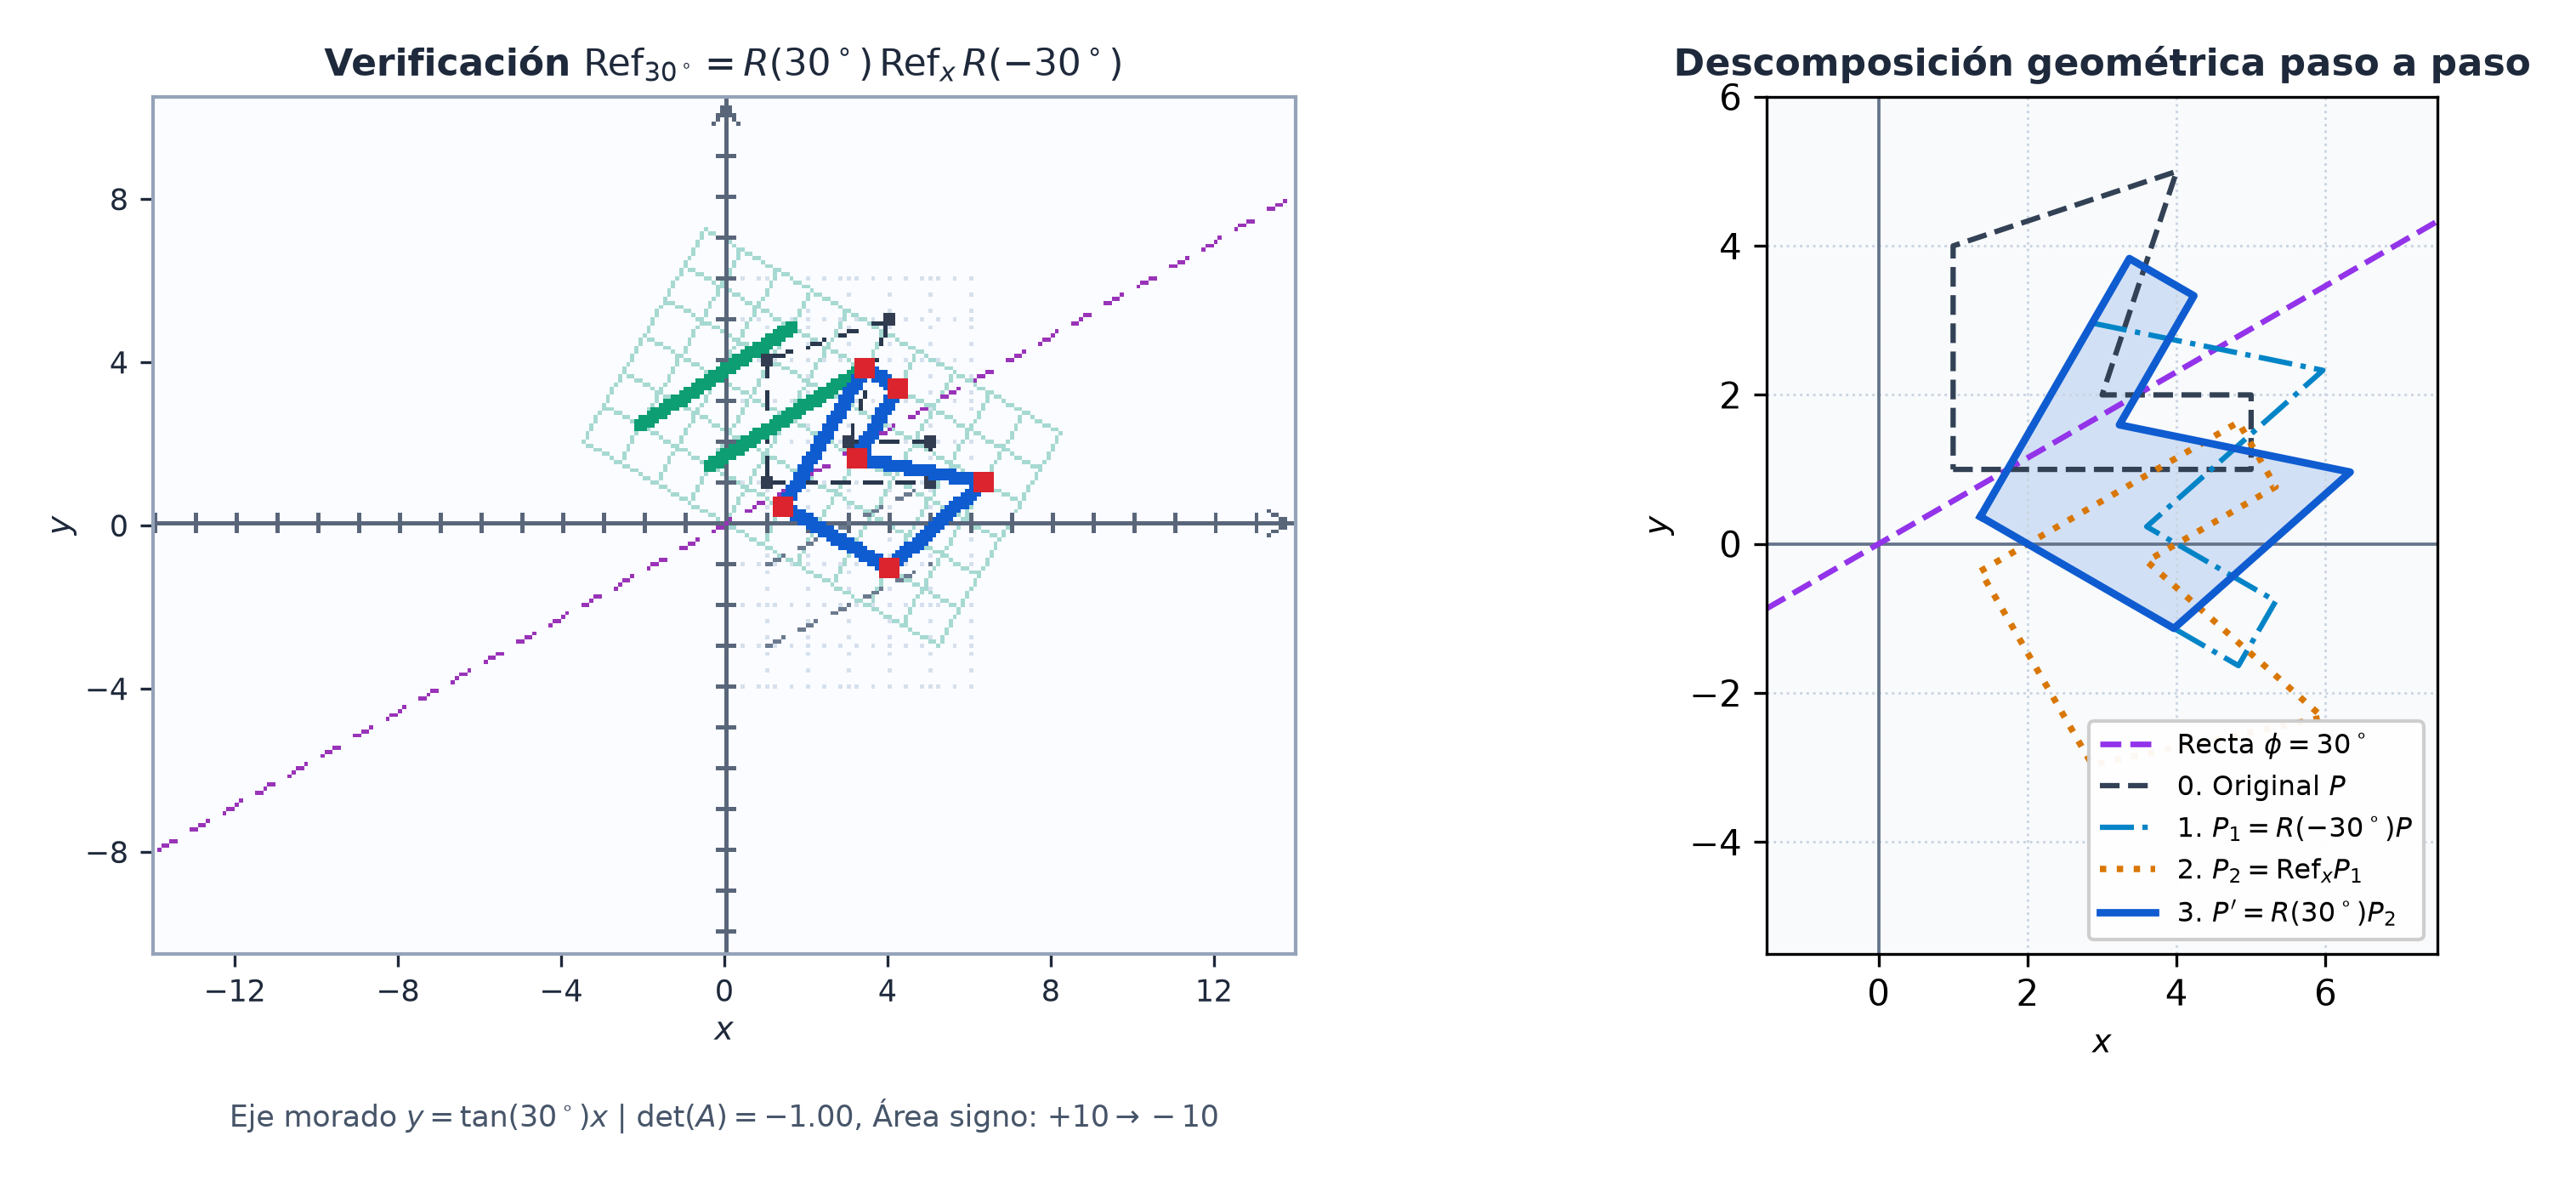
\includegraphics[width=\textwidth]{fig_ref30_steps.png}
  \caption{Verificación visual de $\mathrm{Ref}_{30^\circ} = R(30^\circ)\,\mathrm{Ref}_x\,R(-30^\circ)$: salida raster real del programa C++ (izquierda) y descomposición geométrica paso a paso (derecha).}
  \label{fig:ref30}
\end{figure}

\subsection{Papel de $\det(A)$ e invariantes afines}

Dado un paralelogramo generado por vectores $u,v\in\mathbb{R}^2$, su área con signo es $\det([u\;v])$. Al aplicar la parte lineal $A$, los vectores imagen son $Au$ y $Av$, por lo que:
\begin{equation}
  \det([Au\;\;Av]) = \det(A\,[u\;\;v]) = \det(A)\,\det([u\;\;v]).
\end{equation}
Por triangulación de cualquier polígono simple y linealidad de la traslación, el área con signo escala exactamente por $\det(A)$ \cite{shirley2021}:
\begin{itemize}
  \item \textbf{Factor de área:} $\text{Área}'_{\text{abs}} = |\det(A)| \cdot \text{Área}_{\text{abs}}$.
  \item \textbf{Orientación:} si $\det(A) > 0$ se preserva el sentido de recorrido (CCW $\to$ CCW); si $\det(A) < 0$ la orientación se invierte (CCW $\to$ CW).
  \item \textbf{Invertibilidad:} $M$ es invertible si y solo si $\det(A)\neq 0$, con $M^{-1}$ compuesta por $A^{-1}$ y traslación $-A^{-1}t$. Si $\det(A)=0$, $\mathrm{rango}(A)<2$, el núcleo es no trivial, distintos puntos colapsan en un mismo destino y no existe $M^{-1}$.
\end{itemize}

\textbf{Propiedades conservadas bajo afines invertibles ($\det(A)\neq 0$).}
Sea una recta parametrizada $r(\lambda) = p_0 + \lambda d$. Su imagen es $r'(\lambda) = A(p_0+\lambda d)+t = (Ap_0+t) + \lambda (Ad)$, que es nuevamente una recta no degenerada porque $\det(A)\neq 0 \implies Ad\neq 0$. De ello se deducen directamente cuatro invariantes \cite{foley2014}:
\begin{enumerate}
  \item \emph{Rectas y colinealidad:} puntos sobre una recta permanecen sobre una recta.
  \item \emph{Razones de segmentos colineales:} para $q = (1-\lambda)p_0 + \lambda p_1$, se cumple $q' = (1-\lambda)p'_0 + \lambda p'_1$, preservando puntos medios y proporciones.
  \item \emph{Paralelismo:} si dos rectas tienen directores proporcionales $v = \alpha u$, sus imágenes cumplen $Av = \alpha (Au)$ y permanecen paralelas (y distintas, por inyectividad de $A$).
\end{enumerate}

\textbf{Por qué longitudes y ángulos no se conservan en general (contraejemplo).} Con $H_x(0.7)$, los vectores ortogonales $e_1=(1,0)^T$ y $e_2=(0,1)^T$ se transforman en $e'_1=(1,0)^T$ ($\|e'_1\|=1$) y $e'_2=(0.7,1)^T$ ($\|e'_2\|=\sqrt{1.49}\approx 1.2207 \neq 1$). El ángulo entre ellos pasa de $90^\circ$ a $\arccos(0.7/\sqrt{1.49}) \approx 55.01^\circ$. Longitudes y ángulos solo se conservan cuando $A$ es ortogonal ($A^T A = I$, isometrías).

% ==============================================================================
\section{Arquitectura e implementación en C++}
% ==============================================================================

El laboratorio se implementó en \textbf{C++17} con CMake, OpenGL 2.1 y GLFW 3 sobre WSL2 (\texttt{Ubuntu} 24.04), compilando sin advertencias bajo \texttt{-Wall -Wextra -Wpedantic}. La arquitectura desacopla por completo la matemática de la visualización para garantizar reproducibilidad y pruebas automatizadas:

\begin{itemize}
  \item \texttt{src/math\_affine.hpp}: define \texttt{Point}, \texttt{Segment}, \texttt{Matrix3}, todas las matrices afines ($T, R, S, H_x, H_y, \mathrm{Ref}_x, \mathrm{Ref}_y, \mathrm{Ref}_\phi$), \texttt{multiplyMatrix}, \texttt{composeInApplicationOrder}, \texttt{transformPoint}, \texttt{linearDeterminant}, \texttt{tryInvertAffine}, \texttt{signedArea} y \texttt{measureParallelism}.
  \item \texttt{src/raster.hpp}: implementa \texttt{RasterCanvas} ($280\times 210$ celdas lógicas para el espacio de mundo $[-14,14]\times[-10.5,10.5]$ a $10$ celdas/unidad) con \texttt{putPixel()}, \texttt{putPoint()}, \texttt{drawLine()} (Bresenham en los ocho octantes con estilos sólido, discontinuo y punteado), \texttt{drawPolygon()}, ejes cartesianos, cuadrícula transformable y exportador \texttt{savePPM()}.
  \item \texttt{src/experiments.hpp}: define la escena base, los presets \texttt{E0}--\texttt{E5} y \texttt{REF30}, y el generador de reportes numéricos.
  \item \texttt{src/main.cpp}: gestiona la ventana GLFW, vuelca únicamente las celdas lógicas del raster (sin usar \texttt{glTranslatef}, \texttt{glRotatef}, \texttt{glScalef}, \texttt{glMultMatrix*} ni \texttt{GL\_POLYGON}), ofrece presets directos (\texttt{0}--\texttt{8}), ajuste de parámetros en vivo (\texttt{A/D}, \texttt{J/L}, \texttt{Z/X}, \texttt{W/S}, \texttt{Q/E}, flechas, \texttt{F}, \texttt{O}) y un constructor en consola (\texttt{C}) para concatenar $N\ge 3$ transformaciones arbitrarias mostrando orden y matriz resultante $3\times 3$.
  \item \texttt{src/test\_experiments.cpp}: ejecutable \emph{headless} sin OpenGL que valida cada aserción matemática de E1--E5 con tolerancia $10^{-9}$ y exporta \texttt{resultados\_e1\_e5.json} y \texttt{resumen\_experimentos.txt}.
\end{itemize}

\textbf{Escena base y métricas cuantitativas.} Se construyó un polígono asimétrico cóncavo de 6 vértices, $V_0=(1,1)$, $V_1=(5,1)$, $V_2=(5,2)$, $V_3=(3,2)$, $V_4=(4,5)$ y $V_5=(1,4)$, cuya área exacta con signo por la fórmula del zapatero es:
\begin{equation}
  A_{\text{signo}} = \frac{1}{2}\sum_{i=0}^{5}(x_i y_{i+1} - x_{i+1} y_i) = +10.000000\text{ u}^2 \quad (\text{recorrido antihorario CCW}).
\end{equation}
Junto al polígono se dibujan una cuadrícula local $[0,6]\times[-4,6]$ y dos segmentos originalmente paralelos $L_1: (1,-1)\to(5,1)$ y $L_2: (1,-3)\to(5,-1)$ con vector director $u=v=(4,2)$ y separación perpendicular $d_\perp = 4/\sqrt{5} \approx 1.7889$. El paralelismo se cuantifica mediante el seno normalizado entre directores:
\begin{equation}
  \sigma(u',v') = \frac{|u'_x v'_y - u'_y v'_x|}{\|u'\|\,\|v'\|} \in [0, 1],
\end{equation}
complementado con la distancia perpendicular entre rectas soporte para distinguir rectas paralelas reales ($\sigma=0,\; d_\perp > 0$) de rectas colapsadas coincidentes ($\sigma=0,\; d_\perp = 0$) o segmentos colapsados a un punto ($\|u'\|<\varepsilon$). Cuando $|\det(A)| < 10^{-9}$, \texttt{tryInvertAffine} retorna \texttt{false} y el programa emite una advertencia explícita de matriz singular.

% ==============================================================================
\section{Experimentación controlada y validación reproducible (E1--E5)}
% ==============================================================================

Todos los experimentos fueron ejecutados y verificados automáticamente con \texttt{test\_experiments} y renderizados con el rasterizador propio de \texttt{lab\_afines}. La Tabla~\ref{tab:resumen} concentra las métricas obtenidas.

\begin{table}[H]
\centering
\caption{Resumen cuantitativo reproducido directamente desde el laboratorio C++ para E0--E5 y $\mathrm{Ref}_{30^\circ}$.}
\label{tab:resumen}
\scriptsize
\renewcommand{\arraystretch}{1.15}
\begin{tabular}{@{}l r r r r c c r r@{}}
\toprule
\textbf{Exp.} & $\det(A)$ & $A'_{\text{signo}}$ & $|A'|$ & $|\det(A)|A_0$ & \textbf{Orient.} & $\sigma(u',v')$ & $d_\perp(L'_1,L'_2)$ & $\angle V_0\,(^\circ)$ \\
\midrule
E0 (Base) & $+1.0000$ & $+10.0000$ & $10.0000$ & $10.0000$ & CCW & $0.0000$ & $1.7889$ & $90.00$ \\
E1 ($H_x(0.7)$) & $+1.0000$ & $+10.0000$ & $10.0000$ & $10.0000$ & CCW & $0.0000$ & $1.3893$ & $55.01$ \\
E2 ($\mathrm{Ref}_y$) & $-1.0000$ & $-10.0000$ & $10.0000$ & $10.0000$ & CW  & $0.0000$ & $1.7889$ & $90.00$ \\
E3a ($R\cdot H_x$) & $+1.0000$ & $+10.0000$ & $10.0000$ & $10.0000$ & CCW & $0.0000$ & $1.3893$ & $55.01$ \\
E3b ($H_x\cdot R$) & $+1.0000$ & $+10.0000$ & $10.0000$ & $10.0000$ & CCW & $0.0000$ & $1.3113$ & $76.23$ \\
E4 (4 pasos) & $+1.2000$ & $+12.0000$ & $12.0000$ & $12.0000$ & CCW & $0.0000$ & $1.2518$ & $46.85$ \\
E5 ($S(1,0)$) & $0.0000$ & $0.0000$ & $0.0000$ & $0.0000$ & Deg. & $0.0000^\dagger$ & $0.0000^\dagger$ & $0.00$ \\
$\mathrm{Ref}_{30^\circ}$ & $-1.0000$ & $-10.0000$ & $10.0000$ & $10.0000$ & CW & $0.0000$ & $1.7889$ & $90.00$ \\
\bottomrule
\multicolumn{9}{@{}l}{\footnotesize $^\dagger$ En E5, $L'_1$ y $L'_2$ colapsan sobre el mismo segmento $(1,0)\to(5,0)$ en el eje $X$ (coincidentes, no paralelos distintos).}
\end{tabular}
\end{table}

\subsection{E1 (Cizallamiento $H_x(0.7)$) y E2 (Reflexión vertical $\mathrm{Ref}_y$)}

\textbf{E1.} Bajo $H_x(0.7)$, cada punto cumple $(x',y')=(x+0.7y,\; y)$. Los segmentos paralelos pasan de $L_1:(1,-1)\to(5,1)$ y $L_2:(1,-3)\to(5,-1)$ a:
\[
  L'_1:(0.300,-1.000)\to(5.700,1.000),\quad L'_2:(-1.100,-3.000)\to(4.300,-1.000),
\]
con vectores directores idénticos $u'=v'=(5.400,\; 2.000)$, obteniendo $\sigma(u',v')=0.000000$ ($\alpha=0^\circ$) y separación $d_\perp=1.3893>0$. El paralelismo y el área ($10.0000\text{ u}^2$, error $0.00$) se conservan exactamente, mientras que el ángulo recto en $V_0$ cae de $90.00^\circ$ a $55.01^\circ$ y las longitudes de los segmentos crecen de $4.4721$ a $5.7585$.

\textbf{E2.} Bajo $\mathrm{Ref}_y=\mathrm{diag}(-1,1,1)$, todos los vértices invierten su abscisa (p. ej. $V_4=(4,5)\mapsto(-4,5)$). La fórmula del zapatero arroja $A'_{\text{signo}}=-10.0000\text{ u}^2$ y $|A'|=10.0000\text{ u}^2$: el área física se conserva intacta, pero la orientación pasa de antihoraria (CCW) a horaria (CW) en coherencia con $\det(\mathrm{Ref}_y)=-1$.

\begin{figure}[H]
  \centering
  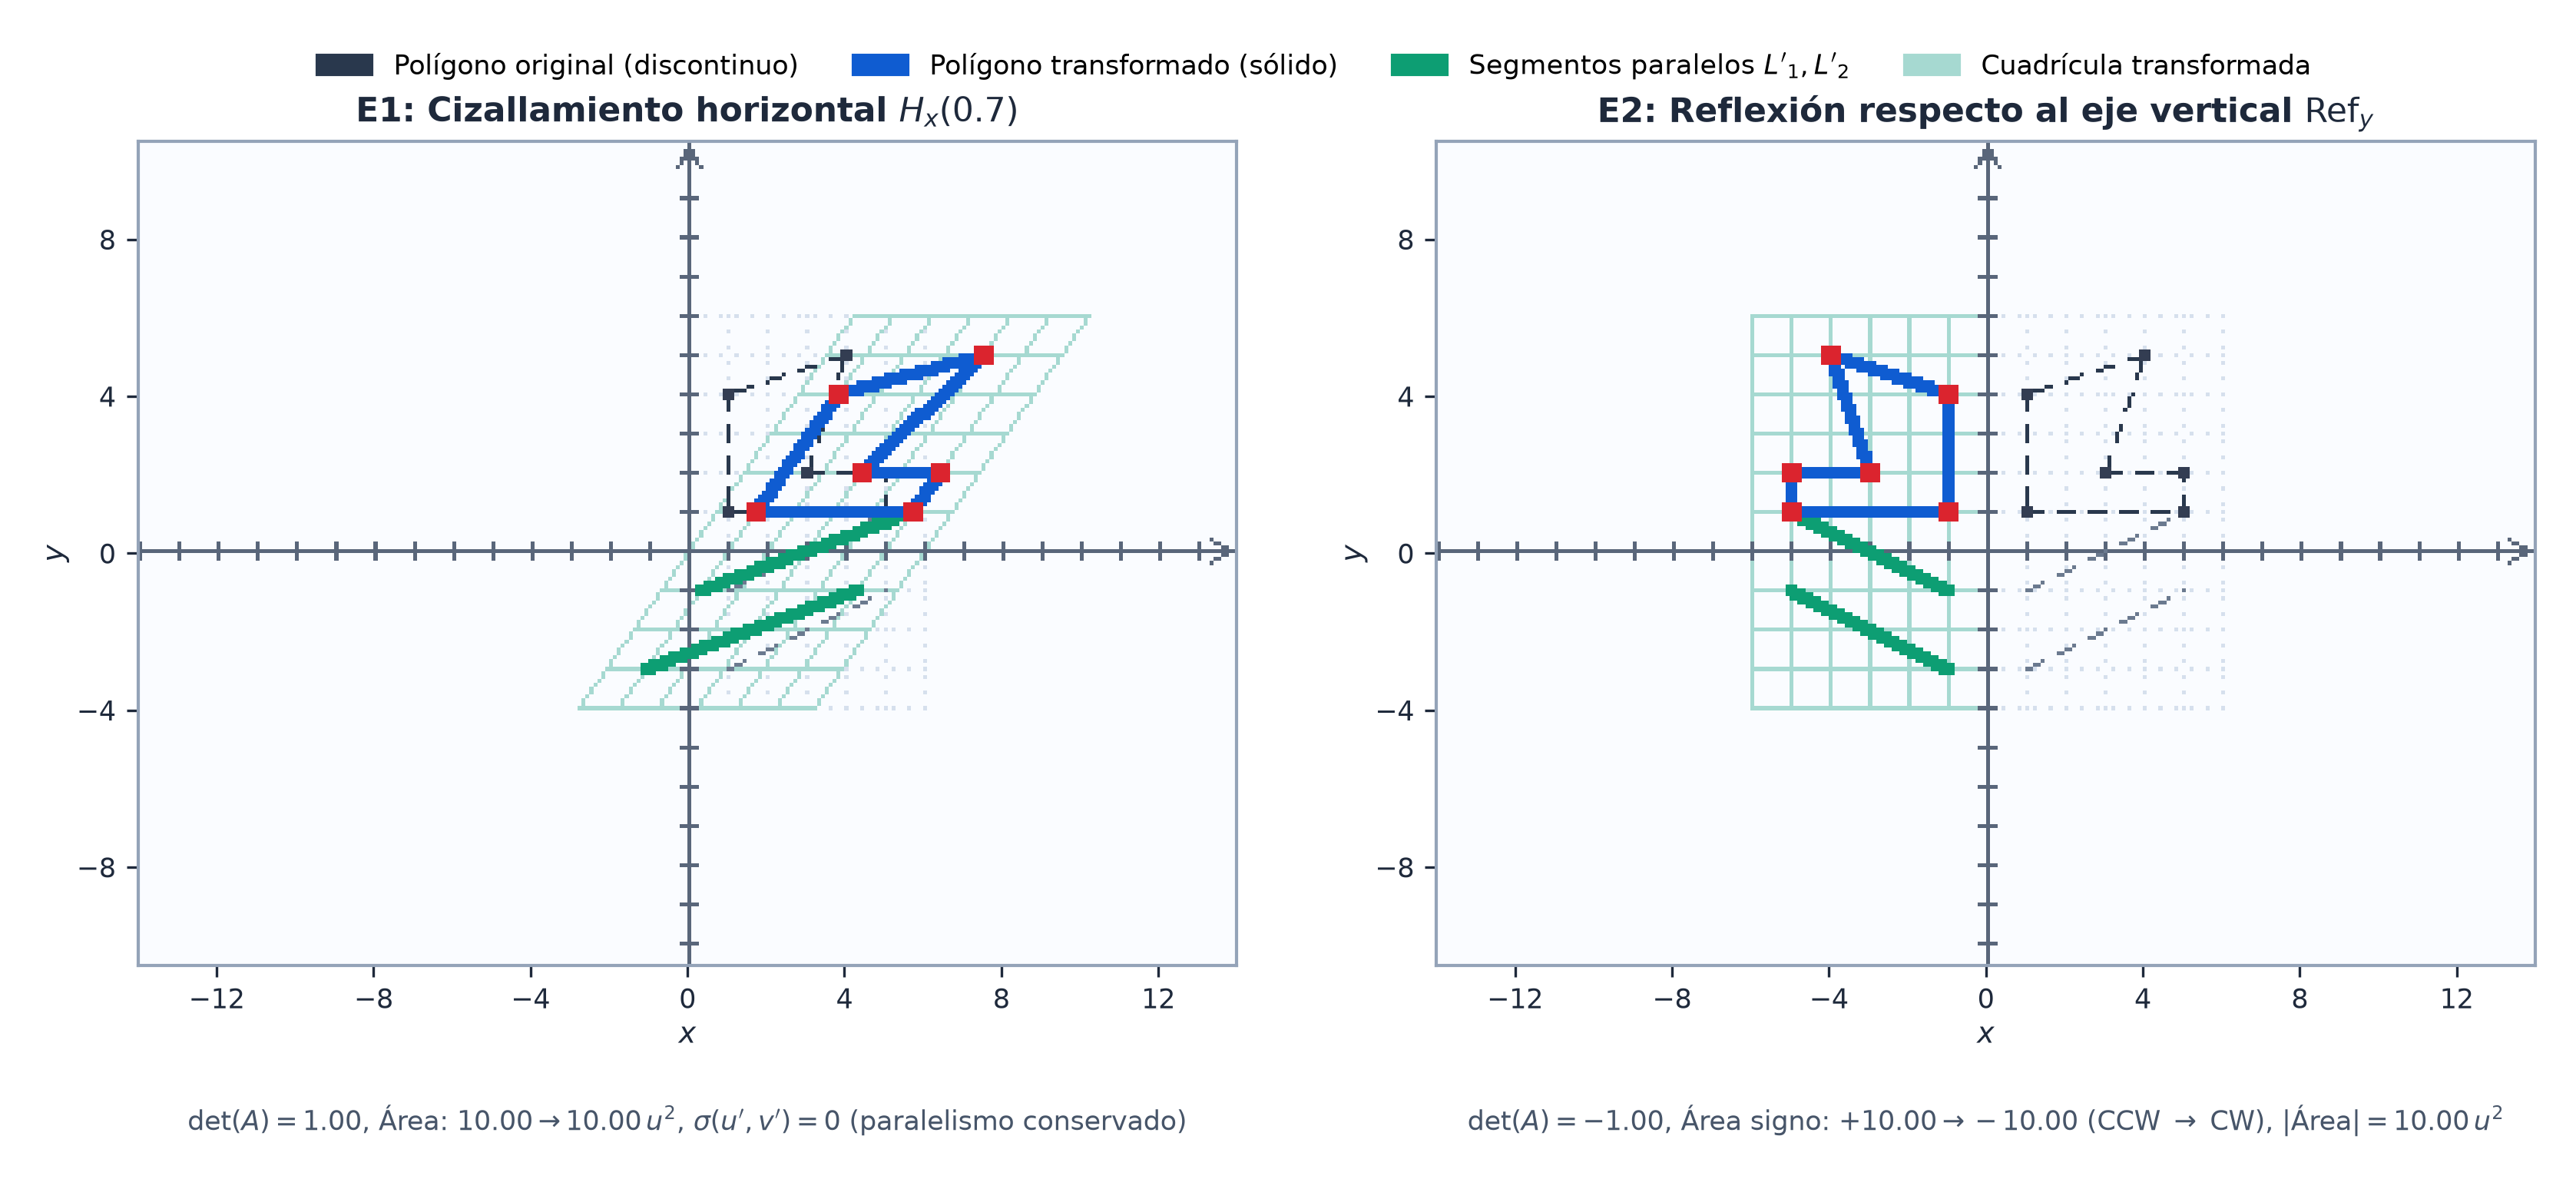
\includegraphics[width=\textwidth]{fig_e1_e2.png}
  \caption{Capturas reales del rasterizador C++ para E1 (izquierda: $H_x(0.7)$) y E2 (derecha: $\mathrm{Ref}_y$). Línea discontinua: figura original; línea azul sólida: figura transformada; verde: segmentos $L'_1, L'_2$.}
  \label{fig:e1e2}
\end{figure}

\subsection{E3: No conmutatividad del orden ($R(45^\circ)H_x(0.7)$ vs. $H_x(0.7)R(45^\circ)$)}

Se comparan las matrices compuestas resultantes:
\begin{equation}
  M_{3a} = R(45^\circ)H_x(0.7) = \begin{bmatrix} 0.7071 & -0.2121 & 0 \\ 0.7071 & 1.2021 & 0 \\ 0 & 0 & 1 \end{bmatrix},
  \qquad
  M_{3b} = H_x(0.7)R(45^\circ) = \begin{bmatrix} 1.2021 & -0.2121 & 0 \\ 0.7071 & 0.7071 & 0 \\ 0 & 0 & 1 \end{bmatrix}.
\end{equation}
Contraste manual en el vértice elegido $V_4 = (4, 5)^T$ (usando $\frac{\sqrt{2}}{2} \approx 0.707107$):
\begin{itemize}
  \item \textbf{Orden 1 ($M_{3a}V_4$, primero $H_x$ luego $R$):} $H_x(0.7)(4,5) = (7.5, 5.0)$; luego $R(45^\circ)(7.5,5.0) = (\frac{\sqrt{2}}{2}(7.5-5.0),\;\frac{\sqrt{2}}{2}(7.5+5.0)) = (1.7678,\; 8.8388)$.
  \item \textbf{Orden 2 ($M_{3b}V_4$, primero $R$ luego $H_x$):} $R(45^\circ)(4,5) = (-\frac{\sqrt{2}}{2},\; 9\frac{\sqrt{2}}{2}) = (-0.7071,\; 6.3640)$; luego $H_x(0.7)$ suma $0.7\times 6.3640$ a $x$, dando $(3.7477,\; 6.3640)$.
\end{itemize}
La discrepancia euclidiana cuantificada en $V_4$ es $\|V'_4 - V''_4\| = \sqrt{(1.7678-3.7477)^2 + (8.8388-6.3640)^2} = \mathbf{3.1694\text{ u}}$, además de diferir en el ángulo en $V_0$ ($55.01^\circ$ vs. $76.23^\circ$) y en la longitud de $V_0V_1$ ($4.0000$ vs. $5.5785$). La Figura~\ref{fig:e3} evidencia el contraste visual y numérico.

\begin{figure}[H]
  \centering
  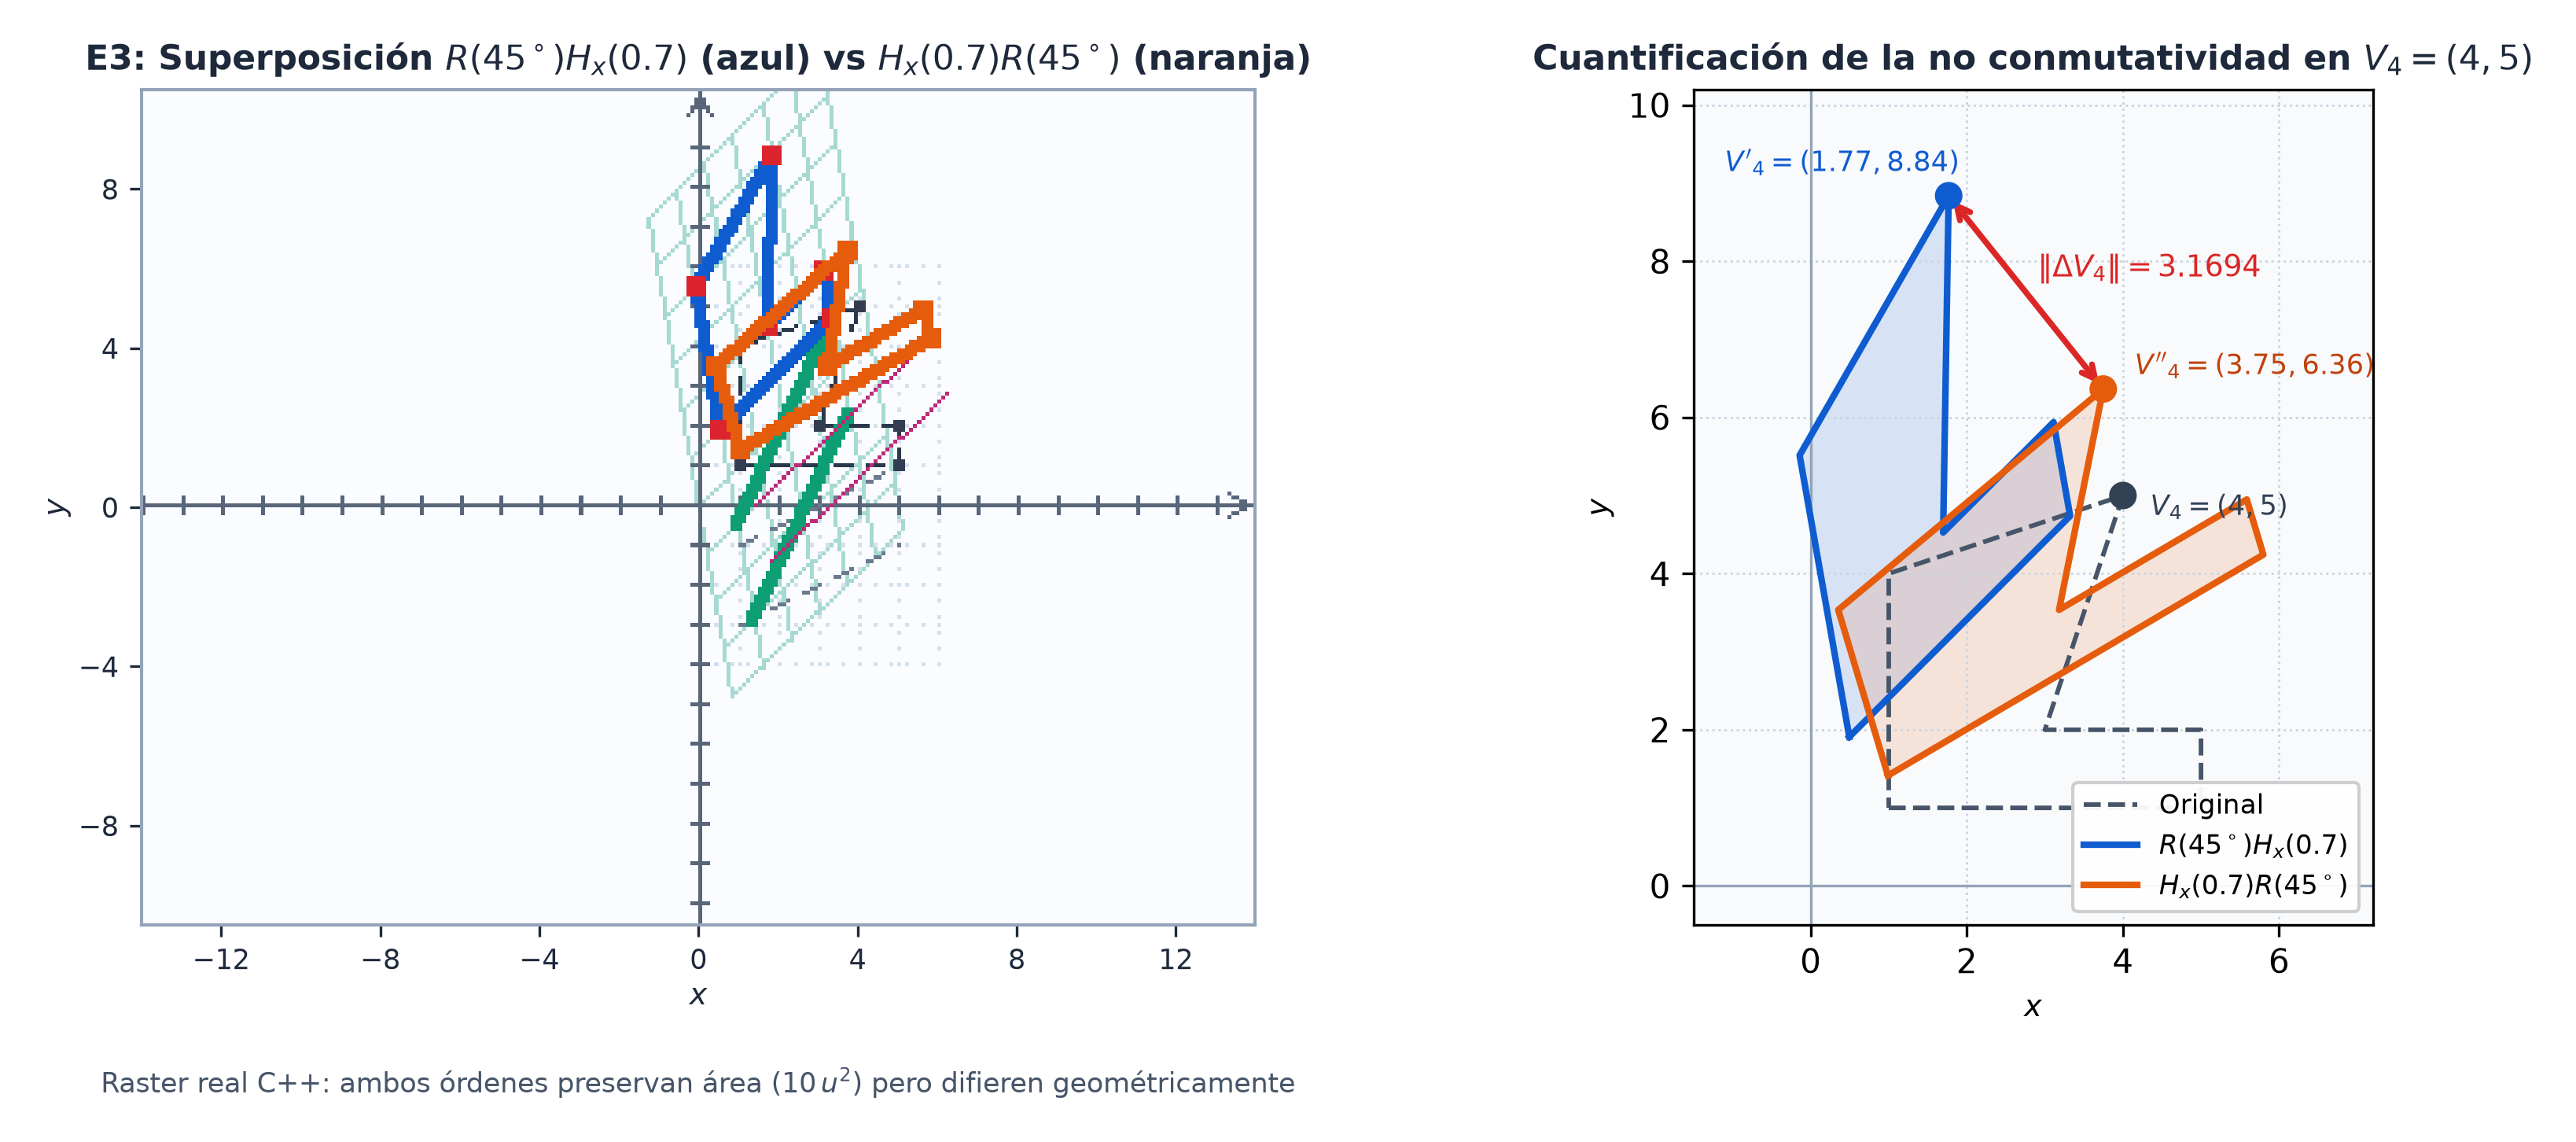
\includegraphics[width=\textwidth]{fig_e3_orden.png}
  \caption{Experimento E3: superposición real del rasterizador C++ (izquierda) y cuantificación de la brecha $\|\Delta V_4\|=3.1694$ en el vértice $V_4=(4,5)$ (derecha).}
  \label{fig:e3}
\end{figure}

\subsection{E4 (Cambio de área) y E5 (Caso degenerado singular)}

\textbf{E4.} Se concatena una cadena de cuatro transformaciones en orden cronológico $H_x(0.5)\to S(1.5,0.8)\to R(25^\circ)\to T(1.5,-1.0)$, cuya matriz compuesta es:
\begin{equation}
  M_{4} = T(1.5,-1.0)\,R(25^\circ)\,S(1.5,0.8)\,H_x(0.5)
  = \begin{bmatrix} 1.3595 & 0.3416 & 1.5000 \\ 0.6339 & 1.0420 & -1.0000 \\ 0 & 0 & 1 \end{bmatrix},
  \quad \det(A_4) = 1.2000.
\end{equation}
El área calculada con la fórmula del zapatero sobre los vértices transformados es $12.000000\text{ u}^2$, coincidiendo con $|\det(A_4)|\cdot A_0 = 1.2 \times 10.0 = 12.000000\text{ u}^2$ con un error numérico de $3.55\times 10^{-15}$ (precisión de máquina IEEE-754). Además, se verificó numéricamente $M_4^{-1}M_4 = I$ mediante \texttt{tryInvertAffine}.

\textbf{E5.} Al aplicar el escalamiento singular $S(1.0, 0.0)$, resulta $\det(A_5)=0$ y cada vértice $(x,y)$ se proyecta a $(x,0)$ sobre el eje $X$. En consecuencia: (i) el polígono pierde su interior y su área colapsa a $0$; (ii) la orientación CCW/CW deja de tener sentido al volverse todos los vértices colineales; (iii) los segmentos $L_1$ y $L_2$, originalmente separados por $1.7889\text{ u}$, colapsan al mismo segmento $(1,0)\to(5,0)$ ($d_\perp=0$), perdiendo la distinción de rectas paralelas; y (iv) la transformación no es inyectiva (infinitos puntos $(x,y)$ con distinto $y$ producen la misma imagen $(x,0)$), por lo que no existe matriz inversa y el programa bloquea su cálculo mostrando la advertencia de singularidad (Figura~\ref{fig:e4e5}).

\begin{figure}[H]
  \centering
  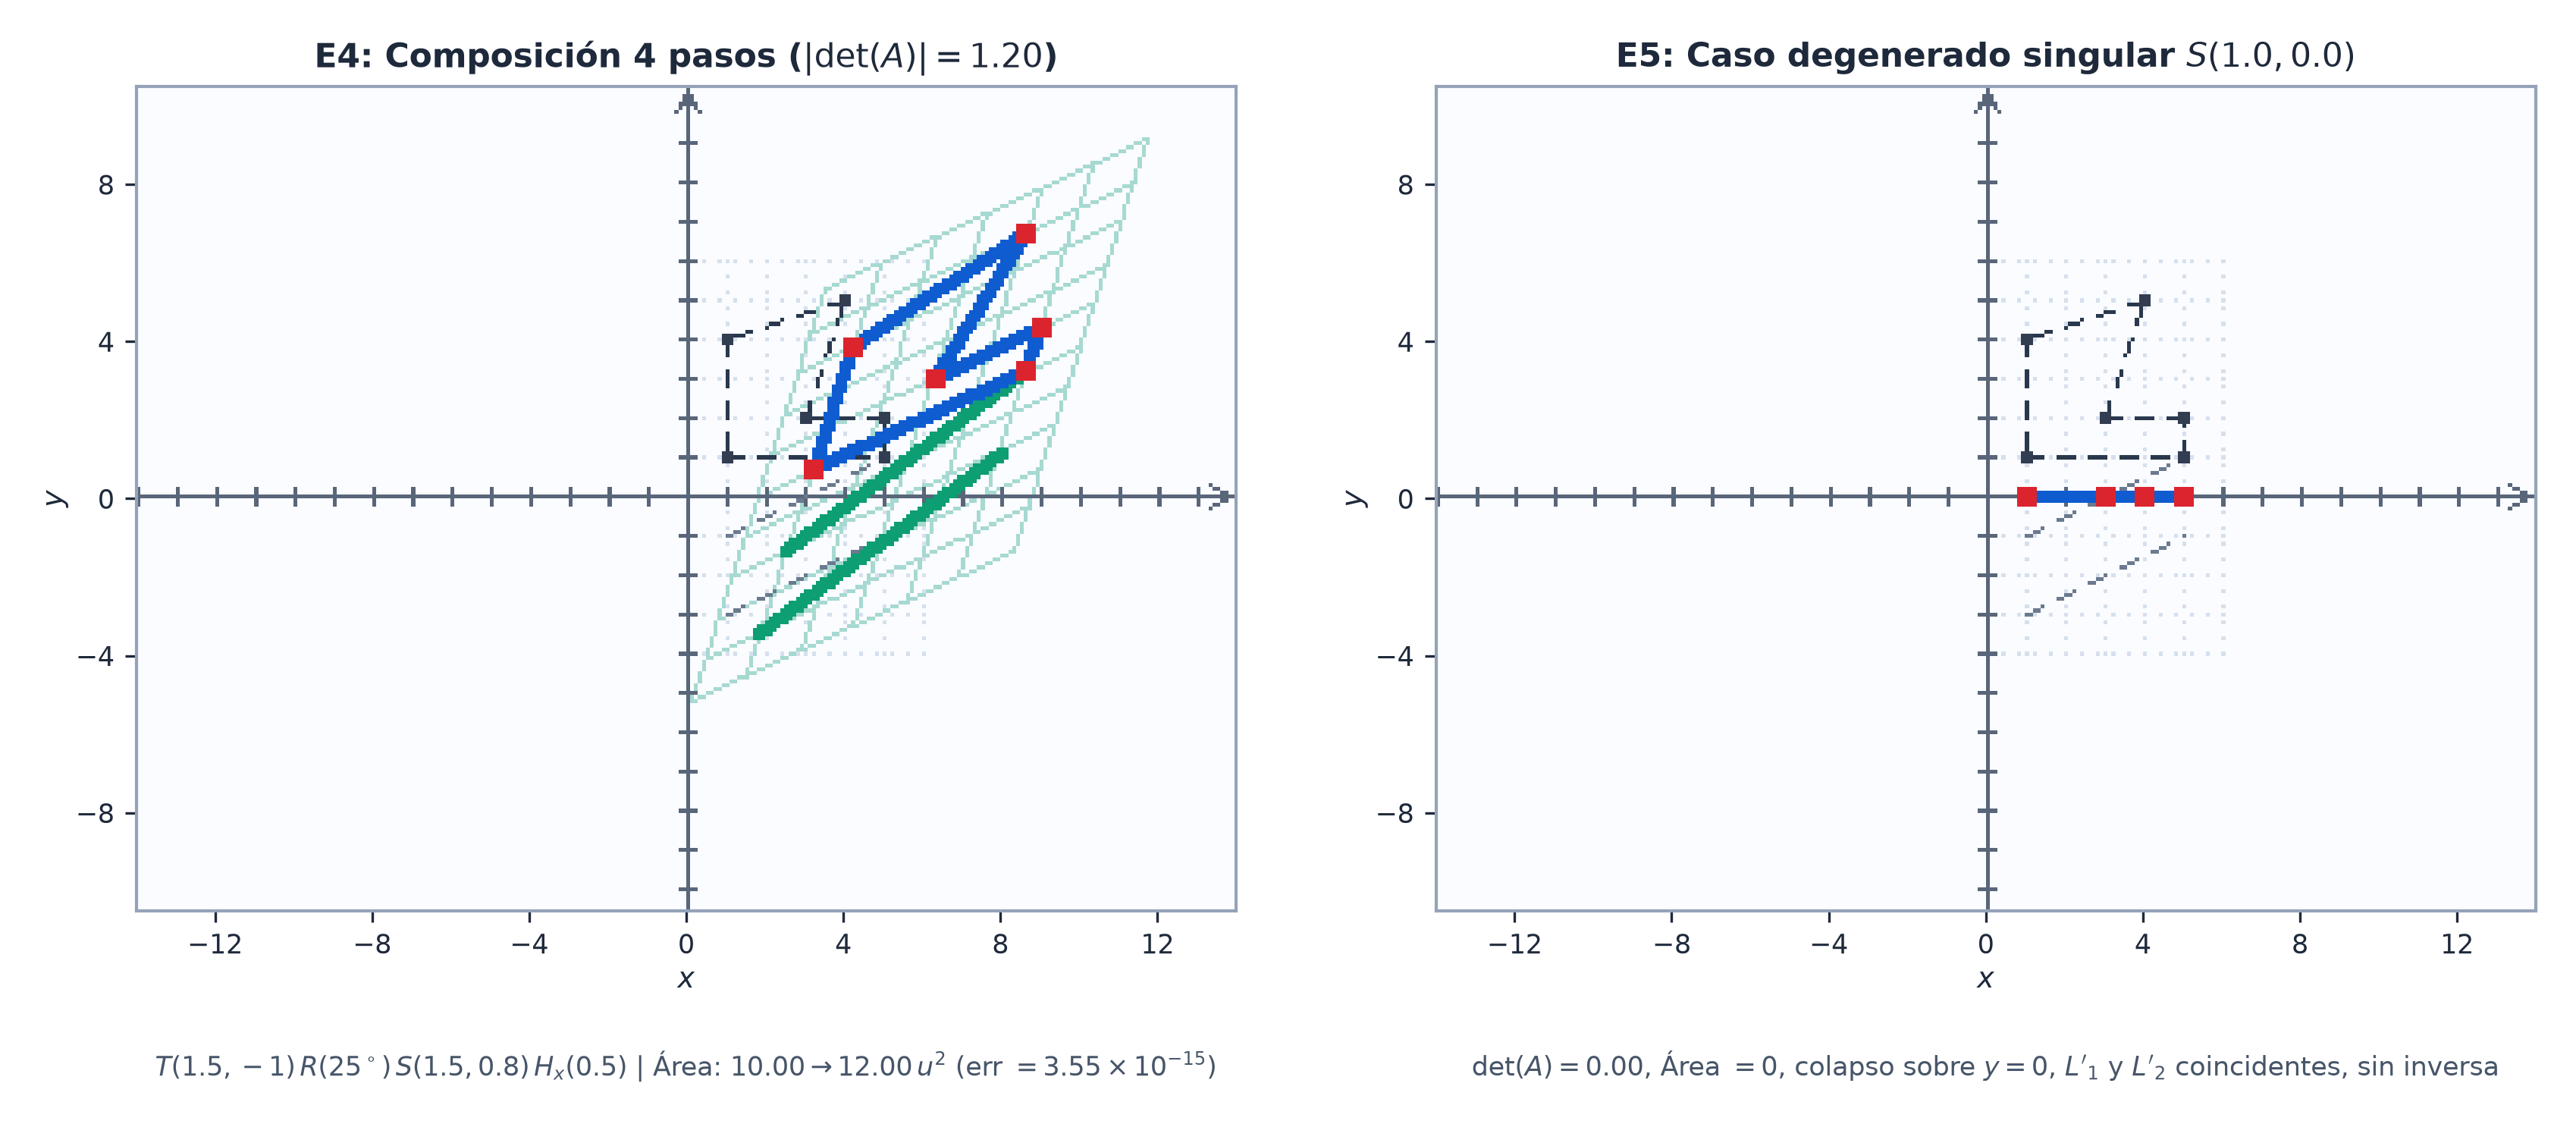
\includegraphics[width=\textwidth]{fig_e4_e5.png}
  \caption{Capturas reales del rasterizador C++ para E4 (izquierda: composición de 4 transformaciones con $|\det(A)|=1.20$) y E5 (derecha: colapso singular sobre $y=0$ bajo $S(1.0,0.0)$).}
  \label{fig:e4e5}
\end{figure}

% ==============================================================================
\section{Análisis, limitaciones y respuestas a las preguntas de defensa}
% ==============================================================================

\textbf{Limitaciones y discretización raster.} Todas las métricas geométricas se calculan en doble precisión (\texttt{double}) antes de rasterizar, logrando errores del orden de $10^{-15}$. Sin embargo, en la visualización discreta mediante Bresenham sobre la rejilla $280\times 210$ ($10$ celdas/unidad), cada vértice continuo se redondea con \texttt{std::lround}, introduciendo una discrepancia puramente visual de hasta $\pm 0.05\text{ u}$ (medio píxel lógico) y efecto escalonado (\emph{aliasing}) en aristas oblicuas. Por ello, las conclusiones nunca se apoyan solo en píxeles sino en los valores analíticos impresos simultáneamente en consola.

\begin{cajaNota}{Respuestas técnicas a las preguntas de defensa (Sección 2.5)}
\begin{enumerate}
  \item \textbf{¿Puede una transformación conservar el área y alterar los ángulos?} \emph{Sí.} Basta que $|\det(A)|=1$ sin que $A$ sea una matriz ortogonal ($A^TA\neq I$). Nuestro experimento E1 ($H_x(0.7)$) lo demuestra: $\det(H_x)=1$ mantiene el área exacta en $10.00\text{ u}^2$, pero el ángulo interno en $V_0$ se deforma de $90.00^\circ$ a $55.01^\circ$. Lo mismo ocurre con un escalamiento anisotrópico equiareal como $S(2, 0.5)$.
  \item \textbf{¿Por qué el determinante negativo no implica área negativa en sentido físico?} Porque en geometría euclidiana el área física (medida de superficie) es siempre no negativa y escala según $|\det(A)|$. El signo de $\det(A)$ codifica la \emph{orientación} (quiralidad) de la base transformada: $\det(A)<0$ indica que el recorrido de los vértices se invirtió de antihorario a horario, tal como muestra E2 ($A'_{\text{signo}}=-10$, $|A'|=10$).
  \item \textbf{¿Por qué una matriz singular requiere un tratamiento especial?} Cuando $\det(A)=0$, la parte lineal reduce la dimensión del plano a una recta o un punto ($\mathrm{rango}(A)<2$): se pierde inyectividad e invertibilidad, el área se anula y propiedades como orientación o ángulos dejan de estar bien definidas. En software, intentar invertirla implica dividir por cero (generando \texttt{NaN}/\texttt{Inf}); por eso debe detectarse con una tolerancia numérica ($|\det(A)|<\varepsilon$) y reportarse sin calcular inversa.
\end{enumerate}
\end{cajaNota}

% ==============================================================================
\section{Conclusiones}
% ==============================================================================

\begin{enumerate}
  \item La implementación explícita de matrices homogéneas $3\times 3$ bajo convención columna ($p'=Mp$) junto con el rasterizador propio (\texttt{putPoint()} y Bresenham) permitió contrastar con precisión de doble flotante ($<10^{-14}$) las predicciones teóricas frente a la deformación visual en todos los casos exigidos.
  \item Los experimentos E1--E4 confirmaron que toda transformación afín invertible preserva el paralelismo ($\sigma=0$) y escala el área con signo por $\det(A)$, pero no conserva ángulos ni longitudes salvo en isometrías; asimismo, E3 cuantificó la no conmutatividad matricial con una brecha de $3.1694\text{ u}$ en $V_4$.
  \item El experimento E5 demostró que la singularidad ($\det(A)=0$) exige un tratamiento diferenciado tanto matemático como computacional, pues colapsa áreas, funde rectas paralelas en rectas coincidentes e invalida la existencia de transformación inversa.
\end{enumerate}

% ==============================================================================
\begin{thebibliography}{9}

\bibitem{hearn2011}
Hearn, D., Baker, M. P., \& Carithers, W. (2011). \emph{Computer Graphics with OpenGL} (4th ed.). Pearson.

\bibitem{foley2014}
Foley, J. D., van Dam, A., Feiner, S. K., \& Hughes, J. F. (2014). \emph{Computer Graphics: Principles and Practice} (3rd ed.). Addison-Wesley.

\bibitem{shirley2021}
Shirley, P., Marschner, S., et al. (2021). \emph{Fundamentals of Computer Graphics} (5th ed.). CRC Press.

\bibitem{vince2012}
Vince, J. (2012). \emph{Mathematics for Computer Graphics} (4th ed.). Springer.

\bibitem{angel2015}
Angel, E., \& Shreiner, D. (2015). \emph{Interactive Computer Graphics: A Top-Down Approach with Shader-Based OpenGL} (7th ed.). Pearson.

\end{thebibliography}

% ==============================================================================
% ANEXOS (no cuentan dentro de las 5-8 paginas del cuerpo)
% ==============================================================================
\newpage
\appendix
\section{Controles del programa, compilación y contribuciones del equipo}

\textbf{Compilación y ejecución reproducibles (Linux / WSL2 Ubuntu).}
Desde la carpeta \texttt{src/}, sin dependencias ocultas ni rutas absolutas:
\begin{verbatim}
cmake -S . -B build && cmake --build build -j
./build/test_experiments ../experimentos
./build/lab_afines
\end{verbatim}

\begin{table}[H]
\centering
\caption{Resumen de controles interactivos implementados en \texttt{lab\_afines}.}
\scriptsize
\renewcommand{\arraystretch}{1.12}
\begin{tabularx}{\textwidth}{>{\bfseries\ttfamily}p{2.3cm} X}
\toprule
Tecla & Acción ejecutada en el laboratorio \\
\midrule
0 -- 8 & Activa los presets E0 (base), E1 ($H_x(0.7)$), E2 ($\mathrm{Ref}_y$), E3a ($RH_x$), E3b ($H_xR$), E3 (superposición), E4 (4 pasos, $|\det|=1.2$), E5 ($S(1,0)$ singular) y $\mathrm{Ref}_{30^\circ}$. \\
I / C & Activa el modo interactivo en vivo ($\ge 3$ transformaciones) o abre el constructor en consola para encadenar $N\ge 3$ transformaciones con parámetros exactos. \\
A, D / J, L & Modifica en vivo el cizallamiento horizontal $k_x$ o vertical $k_y$ ($\pm 0.1$). \\
Z, X / S, W & Modifica en vivo los factores de escala $s_x$ o $s_y$ ($\pm 0.1$; permite llevar $s_y\to 0$ en vivo). \\
Q, E / Flechas & Modifica la rotación $\theta$ ($\pm 5^\circ$) y la traslación $(t_x, t_y)$ ($\pm 0.5$). \\
F / O & Alterna reflexión $\mathrm{Ref}_y$ o invierte el orden de composición de la cadena activa. \\
G / H / P / R & Muestra/oculta cuadrícula, figura original, imprime reporte completo o reinicia parámetros. \\
\bottomrule
\end{tabularx}
\end{table}

\begin{table}[H]
\centering
\caption{Identificación de contribuciones de los integrantes del equipo.}
\scriptsize
\renewcommand{\arraystretch}{1.15}
\begin{tabularx}{\textwidth}{p{5.8cm} X}
\toprule
\textbf{Integrante (Código)} & \textbf{Contribuciones principales} \\
\midrule
CHOQUENAIRA GARCIA, Ronal Franklin (\texttt{174941}) & Formalización matemática (derivación de cizallamiento, reflexiones $\mathrm{Ref}_\phi$ y demostraciones de invariantes), validación de E1--E5, diseño de presentación y demostración en vivo. \\
FERNANDEZ BACA CASTRO, Lucian Neptalí (\texttt{184197}) & Arquitectura e implementación del laboratorio C++17/OpenGL (\texttt{math\_affine.hpp}, \texttt{raster.hpp}, \texttt{main.cpp}, \texttt{test\_experiments.cpp}), automatización de evidencias, informe LaTeX y demostración en vivo. \\
\bottomrule
\end{tabularx}
\end{table}

\end{document}
